%%%%%%%%%%%%%%%%%%%%%%%%%%%%%%%%%%%%%%%%%%%%%%%%%%%%%%%%%%%%%%%%%%%%%%
% How to use writeLaTeX: 
%
% You edit the source code here on the left, and the preview on the
% right shows you the result within a few seconds.
%
% Bookmark this page and share the URL with your co-authors. They can
% edit at the same time!
%
% You can upload figures, bibliographies, custom classes and
% styles using the files menu.
%
%%%%%%%%%%%%%%%%%%%%%%%%%%%%%%%%%%%%%%%%%%%%%%%%%%%%%%%%%%%%%%%%%%%%%%

\documentclass[12pt]{article}

\usepackage{sbc-template}
\usepackage{bm}

\usepackage{graphicx,url}

%\usepackage[brazil]{babel}   
\usepackage[utf8]{inputenc}  
\usepackage{graphicx} % Para inserir imagens
\usepackage{float}    % Para o modificador [H]
\usepackage{booktabs}  % Para tabelas com \toprule, \midrule, \bottomrule

     
\sloppy

\title{Aplicação de Redes Neurais Binarias para a Identificação de Anomalias em Produtos Industriais}

\author{Pedro Henrique Rodrigues da Silva, Marco Tulio Gontijo de Sousa, \\Pedro Henrique Azevedo de Medeiros, Rodrigo de Oliveira Santos }


\address{Curso Ciência de Dados, Pontifícia Universidade Católica de Minas Gerais\\
 Av Dom José Gaspar 500, Belo Horizonte, Minas Gerais, 30535-610}


\begin{document} 

\maketitle


\
\begin{abstract}
  A detecção de anomalias em imagens industriais é um problema crítico para a Indústria 4.0, com aplicações que vão desde a inspeção de qualidade até a manutenção preditiva. No entanto, a implementação de soluções baseadas em deep learning em dispositivos com recursos limitados, como microcontroladores ou GPUs de baixo poder, ainda é um desafio. Este trabalho propõe a aplicação de redes neurais binárias (BNNs) para a detecção de anomalias, visando desenvolver modelos leves e eficientes que possam ser implementados em dispositivos de borda. A relevância do tema é justificada pela necessidade de soluções que combinem alta precisão com baixo custo computacional, além de sua aplicabilidade em cenários industriais reais.
\end{abstract}
\vspace{2cm}

\section{Contextualização}
A Indústria 4.0 tem impulsionado a adoção de tecnologias como Internet das Coisas (IoT) e Inteligência Artificial (IA) para otimizar processos e melhorar a qualidade dos produtos \cite{wang2018industrial}. Nesse cenário, a detecção de anomalias em imagens industriais desempenha um papel crucial, permitindo a identificação precoce de defeitos em produtos e reduzindo custos operacionais \cite{bergmann2019mvtec}. No entanto, a implementação de modelos tradicionais de deep learning em dispositivos com recursos limitados, como microcontroladores ou GPUs de baixo poder, ainda é um desafio significativo \cite{liu2020bidet}.

Redes neurais binárias (BNNs) surgem como uma solução promissora para esse problema, oferecendo eficiência computacional e leveza ao representar pesos e ativações com valores binários (1 ou -1) \cite{courbariaux2015binaryconnect}. Essa abordagem reduz drasticamente o uso de memória e o custo computacional, tornando-a ideal para aplicações em dispositivos de borda \cite{rastegari2016xnet}. No entanto, a binarização pode levar à perda de precisão, especialmente em tarefas complexas como a detecção de anomalias \cite{bulat2020binary}.

Este trabalho propõe a aplicação de redes neurais binárias para a detecção de anomalias em imagens industriais, visando desenvolver modelos leves e eficientes que possam ser implementados em cenários reais. A relevância do tema é justificada pela necessidade de soluções que combinem alta precisão com baixo custo computacional, além de sua aplicabilidade em cenários industriais reais. A contribuição esperada é avançar o estado da arte em BNNs para aplicações de visão computacional, oferecendo uma solução viável para a indústria moderna.

\subsection{Redes Neurais Binárias}
Através da necessidade de compressão das redes neurais convolucionais para uso em máquinas convencionais, uma das técnicas que surge como uma solução promissora e rápida é a quantização da rede de pesos e a binarização é a forma mais extrema de realizar essa técnica. Binarização é a técnica onde os dados são convertidos de pontos flutuantes para terem apenas dois valores possíveis: -1(0) ou +1. Isso evita a extensa carga computacional das multiplicações de matrizes de pesos de dados de pontos flutuantes, além de salvar memória, energia e aumentar significativamente a velocidade de treinamento \cite{bulat2020binary}.

Em uma rede convolucional tradicional, a operação básica é expressa como:
\[z = \sigma (w \otimes a)\]

Onde \textbf{w} e \textbf{a} representam o tensor de pesos e o tensor de ativação gerado pela camada anterior, respectivamente. \textbf{$\sigma$} é a função não linear, \textbf{$\otimes$} representa a função de convolução e \textbf{z} o tensor de saída.
A definição popular de uma função de binarização é a seguinte:
\[Q_w(\bm{w}) = \alpha \bm{b_w},\qquad Q_a (\bm{a}) = \beta \bm{b_a}\]

Onde $\bm{b_w}$ e $\bm{b_a}$ são tensores de pesos binários e ativações binárias, com os respectivos escalares $\alpha$ e $\beta$. 
Com as binarizações, o vetor de multiplicação na propagação direta pode ser reformulado da seguinte maneira:
\[ z = \sigma (Q_w(\bm{w}) \otimes Q_a (\bm{a}))= \sigma(\alpha \beta(\bm{b_w} \odot \bm{b_a}))\]
Onde $\odot$ representa o produto interno para vetores com operações XNOR.
No caso da binarização, a propagação retrógrada leva ao desaparecimento do gradiente, devido aos valores serem restritos a 1 e 0. Sendo assim, uma técnica chamada estimador direto, tradução de \textit{straight-trgough estimator} (STE) proposta por Hinton \textit{et. al.} resolve o problema do gradiente no treinamento de uma rede binária profunda. A STE é definida como:
\[ clip(x, -1, 1) = max(-1, min(1, x))\]
Entretanto, a binarização irá causar um desvio severo de precisão. Mesmo com técnicas apropriadas para aplicação do gradiente descendente, a rede binária falha em retornar uma solução satisfatória.
Esse trabalho irá seguir, a princípio, a abordagem utilizada por \cite{McDonnell2018}

\subsection{Embeddings}

Embeddings de imagens são representações matemáticas que traduzem características visuais de uma imagem em vetores numéricos de alta dimensão. Esses vetores capturam informações como formas, cores, texturas e até mesmo contextos semânticos, permitindo que algoritmos de aprendizado de máquina processem e analisem imagens de maneira eficiente.

A necessidade de utilizar embeddings de imagens surge especialmente em cenários onde o volume de dados visuais é grande e a análise manual seria inviável. Eles permitem que sistemas automatizados processem imagens de forma escalável e eficiente. A técnica começou a ser amplamente utilizada com o advento de arquiteturas como AlexNet e VGGNet, que demonstraram a eficácia das CNNs em extrair características visuais relevantes. Desde então, modelos mais avançados, como ResNet e EfficientNet, têm refinado a criação de embeddings, tornando-os mais precisos e compactos.

Um embedding de imagem é um vetor de números que representa uma imagem em um espaço multi-dimensional. Cada número no vetor corresponde a um atributo da imagem, por exemplo, cor, forma, textura, etc. O vetor captura a essência da imagem e nos permite comparar com outras imagens. Embeddings também são muito conhecidos como descritores de imagem. 

Os embeddings consistem nas principais características da imagem. Quando não existe um número fixo de classes, quando temos muitas classes, quando queremos comparar imagens ou agrupar ou ranquear imagens mais parecidas, os embeddings são muito utilizados.

\subsubsection{HOG (\textit{Histogram of Oriented Gradients)}}
Desenvolvido por Dalal e Triggs, o Histograma de Gradientes Orientados é um descritor cuja função se dá através da distribuição (histograma) de gradientes orientados de uma imagem. O HOG é capaz de extrair bordas de um ou mais objetos, para depois enviá-las a um algoritmo classificador responsável por definir, por exemplo, se na imagem analisada há ou não uma face \cite{DilermandoErick2022}.

Gradientes representam a mudança de tonalidade no decorrer da foto em uma orientação. Normalmente, uma mudança abrupta de cor em uma foto representa uma mudança de objeto ou fundo.

Além do HOG, muitos outros descritores se baseiam no uso de gradientes orientados na detecção de objetos; entretanto, este e alguns outros algoritmos utilizam uma técnica chamada contexto de forma (\textit{Shape of Context}, que é a divisão da imagem em blocos para conseguir extrair as bordas de um objeto. Dalal e Triggs se basearam nessa proposta para aplicar um histograma de gradientes orientados em cada célula dessa, distinguindo HOG dos demais descritores \cite{DilermandoErick2022}.

\subsubsection{LBP (\textit{Local Binary Patterns)}}
Para explicar o LPB deve-se ter em mente o que é textura em uma imagem. Textura é definida pelas relações locais entre os pixels de uma imagem e capturada por meio de padrões binários. Esses padrões descrevem a variação de intensidade ao redor de cada pixel central e formam a base para a identificação das características texturais da imagem. Desta maneira, o cálculo do operador LBP pode ser visualizado na imagem~\ref{fig:LBPembedding}, onde o pixel central comanda a binarização das células ao redor. Aqueles maiores ou iguais ao valor central são convertidos em 1; caso contrário, 0. O código binário LBP deste pixel central é composto dessas marcações de maneira anti-horária. Ao final, o padrão binário é obtido convertendo o código binário em decimal \cite{LBP}\cite{FaceRocgnition}.

\begin{figure}[H]
    \centering
    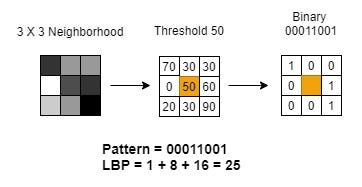
\includegraphics[width=0.75\linewidth]{1_FLFCkrSCgrf4Ps-NmW1OXQ.jpeg}
    \caption{Representação de uma etapas para extração do valor do descritor LBP.}
    \label{fig:LBPembedding}
\end{figure}

Como pode ser visto na imagem~\ref{fig:LBPembedding}, a grade 3x3 é o padrão para a ideia inicial da abordagem. Esse operador não é tão robusto em relação às variações de textura, causadas, por exemplo, por ponto de vista ou direção de iluminação. As variáveis calculadas em um raio 3x3 não capturam estruturas em larga escala. Dessa maneira, para contrapor essa deficiência, é introduzido o operador multi-resolução LBP.

O operador LBP multi resolução \cite{LBP} recebe como  parâmetro para cálculo o raio R de um círculo e os P pixels uniformes contidos neste, como mostra a figura~\ref{fig:3LBPoperator}. Desta maneira, a influência de P e R devem ser consideradas na performance do operador. Operadores com mais labels produz um histograma longo e uma matriz de distâncias computacionalmente díficil de calcular, por outro lado, um menor número de labels resulta na falta de informação \cite{FaceRocgnition}.

\begin{figure}[H]
    \centering
    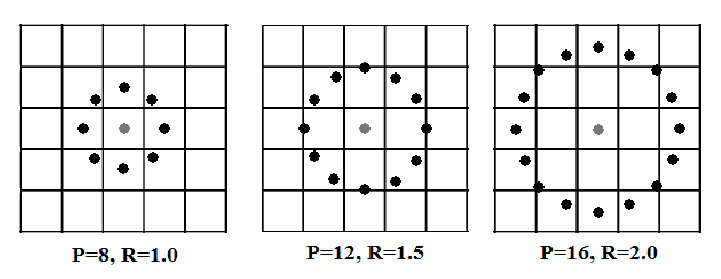
\includegraphics[width=0.75\linewidth]{Multi-scale-LBP-operator.png}
    \caption{Três operadores LBP circulares simétricos com diferentes raios.}
    \label{fig:3LBPoperator}
\end{figure}


\section{Metodologia}
\subsection*{Etapa 1 – Extração e Avaliação de Embeddings}

A primeira etapa deste trabalho, ilustrada de forma esquemática na Figura~\ref{fig:infografico_pipeline}, envolveu a padronização e representação vetorial das imagens industriais por meio de diferentes técnicas de extração de embeddings. Inicialmente, foi realizada a padronização das imagens de entrada, com o objetivo de uniformizar as dimensões e o formato dos dados visuais. Essa etapa foi fundamental para garantir que os descritores operassem de maneira consistente e comparável.

Na sequência, as imagens foram submetidas a três métodos distintos de extração de características, previamente descritos na Seção 1.2: \textbf{HOG (Histogram of Oriented Gradients)}, \textbf{LBP (Local Binary Patterns)} e \textbf{Binary ResNet}. Cada imagem foi convertida em um vetor de características de alta dimensão por cada uma dessas abordagens. 

Os embeddings obtidos foram posteriormente submetidos à técnica de redução de dimensionalidade \textbf{UMAP (Uniform Manifold Approximation and Projection)}, com o objetivo de projetar os dados em um espaço bidimensional, facilitando a visualização da separação entre as classes.

A qualidade da separação entre os grupos foi quantificada utilizando a métrica de \textbf{Silhouette Score}, que avalia o grau de coesão intraclasse e de separação entre classes distintas. A Tabela~\ref{tab:avaliacao_embeddings} apresenta os valores médios obtidos para cada uma das técnicas de embedding.

\begin{table}[H]
\centering
\caption{Avaliação dos embeddings com base na métrica de Silhouette Score}
\label{tab:avaliacao_embeddings}
\begin{tabular}{lcc}
\toprule
\textbf{Técnica de Embedding} & \textbf{Silhouette Score médio} & \textbf{Desvio padrão} \\
\midrule
HOG         & 0.32 & 0.04 \\
LBP         & 0.41 & 0.05 \\
Binary ResNet & 0.62 & 0.03 \\
\bottomrule
\end{tabular}
\end{table}

A Figura~\ref{fig:umap_comparacao} ilustra as projeções geradas com UMAP para os três métodos, permitindo uma comparação visual direta do poder de separação de classes entre os embeddings.

\begin{figure}[H]
\centering
\includegraphics[width=\textwidth]{comparação.png}
\caption{Projeção UMAP para os três métodos de embedding: HOG, LBP e Binary ResNet}
\label{fig:umap_comparacao}
\end{figure}

Dentre os métodos avaliados, a \textbf{Binary ResNet} apresentou o melhor desempenho, com maior separabilidade entre as classes e valores superiores de Silhouette Score. Essa evidência fundamenta sua escolha como técnica principal para as próximas etapas do pipeline, voltadas à detecção e classificação de anomalias.

\begin{figure}[H]
\centering
\includegraphics[width=0.85\textwidth]{embeddings.png}
\caption{Fluxo metodológico geral para extração e avaliação de embeddings}
\label{fig:infografico_pipeline}
\end{figure}


\vspace{2cm}
\newpage
\bibliographystyle{sbc}
\bibliography{sbc-template}

\end{document}
